%% ANT LABS Technical Documentation		
%% Software Manual and Technical Document Template	
%% 									
%% This provides an example of a software manual created in Overleaf.

\documentclass{ol-softwaremanual}
%---- Required Packages and Functions ----

\usepackage{graphicx}  % For including images
\usepackage{fancyhdr}  % For custom headers and footers
\usepackage{microtype} % For typographical enhancements
\usepackage{minted}    % For code listings
\usepackage{amsmath}   % For equations and mathematics
\usepackage{hyperref}  % For hyperlinks
\usepackage[utf8]{inputenc}
\usepackage{graphicx}  % For including images
\usepackage{fancyhdr}  % For custom headers and footers
\usepackage{microtype} % For typographical enhancements
\usepackage{minted}    % For code listings
\usepackage{amsmath}   % For equations and mathematics
\usepackage{hyperref}  % For hyperlinks
\usepackage{array}           % For table customization
\usepackage{booktabs}        % For better table lines
\usepackage{tikz}
\usetikzlibrary{er}
% Set page size and margins
\usepackage[a4paper,top=3cm,bottom=3cm,left=2cm,right=2cm,headheight=50pt,headsep=20pt]{geometry}

% Custom header
\pagestyle{fancy}
\fancyhf{}  % Clear all header and footer fields
\fancyhead[L]{%
   \textit{Relazione Basi di Dati}
}

% Custom footer
\fancyfoot[L]{%
  \parbox{16.7cm}{%
    \centering \thepage
  }
}

% Custom macros used in this example document
\newcommand{\doclink}[2]{\href{#1}{#2}\footnote{\url{#1}}}
\newcommand{\cs}[1]{\texttt{\textbackslash #1}}


% Frontmatter data; appears on title page
\title{Relazione Progetto \\Basi di Dati}
\version{1.0.0}
\author{Simone Acuti \& Alessio Ganzarolli}
% Define a page style with logo
\softwarelogo{
\includegraphics[width=6cm]{unife_logo.png}}

\begin{document}

\maketitle

\tableofcontents
\newpage

\section{Pulizia dei dati}

Gli script per la pulizia dei dati sono stati racchiusi nella directory src/python, e si compone dei seguenti file:
\begin{itemize}
    \item \textbf{clean\_artist\_data.py}: passaggi per pulire il dataset artist;
    \item \textbf{clean\_artwork\_data.py}: passaggi per pulire il dataset artwork;
    \item \textbf{common.py}: funzioni comuni per la pulizia e altri scopi;
    \item \textbf{constants.py}: costanti utili, quali percorsi di file e valori di default per gli attributi;
    \item \textbf{main.py}: script per eseguire entrambe le pulizie in modo concorrente;
\end{itemize}
Ogni operazione di pulizia eseguita viene illustrata nel dettaglio all’utente tramite il terminale.

\subsection{Pulizia dataset artist}
Il dataset presentava dati molto grezzi che meritavano una pulita. Più nel dettaglio:
\begin{itemize}
    \item Sostituzione dei valori Male e Female della colonna \verb|gender| con M ed F.
    \item Rimozione della colonna \verb|dates| per ridondanza, in quanto i valori al suo interno erano già presenti 
    nelle colonne \verb|yearOfBirth| e \verb|yearOfDeath|;
    \item Scissione della colonna \verb|placeOfBirth| in \verb|cityOfBirth| e \verb|stateOfBirth|, e della colonna \verb|placeOfDeath| in 
    \verb|cityOfDeath| e \verb|stateOfDeath|;
    \item Operazioni comuni elencate più sotto.
\end{itemize}

\subsection{Pulizia dataset artwork}
Anche questo dataset era colmo di valori ridondanti e dati consistenti, di conseguenza sono state effettuate le seguenti operazioni:
\begin{itemize}
    \item Rimozione di alcuni valori inappropriati (c., (upper), (each)…);
    \item Rimozione delle colonne \verb|artist|, \verb|dateText| e \verb|dimensions| per ridondanza;
    \item Riparazione dei link alle immagini delle opere sostituendo \verb|www| con \verb|media|;
    \item Operazioni comuni elencate più sotto;
    \item Rimozione di 6 righe in quanto il loro valore di \textbf{Foreign Key} non era presente nella colonna referenziata del database artist.
\end{itemize}

\newpage
\subsection{Operazioni comuni}
Alcune operazioni di pulizia sono state eseguite ad entrambi i dataset:
\begin{itemize}
    \item Gestione di tutti i valori mancanti inserendo al loro posto dei valori di default per ogni colonna collocati nel 
    file \textbf{constants.py};
    \item Ordinamento tramite colonna \verb|id|;
    \item Conversione di eventuali nomi di attributi dal camelCase allo snake\_case;
\end{itemize}

\section{Query SQL}

Siccome le pagine dei punti 1 e 3 comportano l'utilizzo di molti filtri, vi è la necessità di creare una query per ogni tag. Dato che hanno la stessa 
struttura, possiamo scriverne una unica che viene chiamata più volte iterando su un array contenente i nomi degli attributi (indicate con *).

\subsection{Punto 1}
\begin{itemize}
    \item Riempimento tag select con i nomi degli artisti:
    \begin{minted}{sql}
    SELECT name
    FROM artist
    ORDER BY name
    \end{minted}
    \item *Riempimento dei rimanenti tag select per i filtri:
    \begin{minted}{sql}
    SELECT DISTINCT '$attr'
    FROM artist
    ORDER BY '$attr'
    \end{minted}
    La query viene chiamata per gli attributi: \verb|year_of_birth|, \verb|year_of_death|, \\
    \verb|city_of_birth|, \verb|state_of_birth|, \verb|city_of_death|, \verb|state_of_death|.
    \item Risultati della ricerca:
    \begin{minted}{sql}
    SELECT *
    FROM artist
    WHERE (
    name LIKE '%$name%' 
    AND year_of_birth LIKE '%$year_of_birth%'
    AND year_of_death LIKE '%$year_of_death%'
    AND city_of_birth LIKE '%$city_of_birth%' 
    AND state_of_birth LIKE '%$state_of_birth%' 
    AND city_of_death LIKE '%$city_of_death%' 
    AND state_of_death LIKE '%$state_of_death%')
    \end{minted}
\end{itemize}

\subsection{Punto 2}
\begin{itemize}
    \item Riempimento tag select con i nomi degli artisti:
    \begin{minted}{sql}
    SELECT at.name, at.id 
    FROM artist AS at 
    ORDER BY at.name
    \end{minted}
    \item Tabella con dipinti e informazioni:
    \begin{minted}{sql}
    SELECT ak.*, at.name 
    FROM artist AS at, artwork AS ak
    WHERE ak.artist_id='$artist_id'
    AND at.id=ak.artist_id
    LIMIT 500
    \end{minted}
\end{itemize}

\subsection{Punto 3}
\begin{itemize}
    \item Riempimento tag select con i nomi degli artisti:
    \begin{minted}{sql}
    SELECT at.name, at.id
    FROM artist AS at
    ORDER BY at.name
    \end{minted}
    \item *Riempimento dei rimanenti tag select per i filtri:
    \begin{minted}{sql}
    SELECT DISTINCT '$attr' 
    FROM artwork
    ORDER BY '$attr'
    \end{minted}
    La query viene chiamata per gli attributi: \verb|medium|, \verb|year|, \verb|acquisition_year|.
    \item Risultati della ricerca:
    \begin{minted}{sql}
    SELECT *
    FROM artwork
    WHERE (
    artist_id LIKE '%$artist_id%' 
    AND medium LIKE '%$medium%'
    AND year LIKE '%$year%'
    AND acquisition_year LIKE '%$acquisition_year%')
    LIMIT 500
    \end{minted}
\end{itemize}

\newpage
\subsection{Punto 4}
\subsubsection{Statistica 1}
\begin{itemize}
    \item Riempimento tag select con gli anni di creazione di tutti i dipinti:
    \begin{minted}{sql}
    SELECT DISTINCT year 
    FROM artwork
    ORDER BY year
    \end{minted}
    \item Numero di dipinti fatti nell'anno selezionato:
    \begin{minted}{sql}
    SELECT COUNT(*)
    FROM artwork
    WHERE year='$year'
    \end{minted}
\end{itemize}
\subsubsection{Statistica 2}
\begin{itemize}
    \item Riempimento tag select con le nazioni di nascita degli artisti:
    \begin{minted}{sql}
    SELECT DISTINCT state_of_birth 
    FROM artist
    ORDER BY state_of_birth
    \end{minted}
    \item Riempimento tag select con le nazioni in cui gli artisti sono morti:
    \begin{minted}{sql}
    SELECT DISTINCT state_of_death
    FROM artist
    ORDER BY state_of_death
    \end{minted}
    \item Numero di artisti nati nella nazione selezionata:
    \begin{minted}{sql}
    SELECT COUNT(*)
    FROM artist 
    WHERE state_of_birth = '$state_of_birth'
    \end{minted}
    \item Numero di artisti morti nella nazione selezionata:
    \begin{minted}{sql}
    SELECT COUNT(*)
    FROM artist 
    WHERE state_of_death = '$state_of_death'
    \end{minted}
\end{itemize}
\subsubsection{Statistica 3}
\begin{itemize}
    \item Riempimento tag select con i nomi degli artisti:
    \begin{minted}{sql}
    SELECT name
    FROM artist
    ORDER BY name
    \end{minted}
    \newpage
    \item Numero di dipinti fatti dall'artista selezionato:
    \begin{minted}{sql}
    SELECT name, COUNT(*)
    FROM artist, artwork 
    WHERE artist.id=artwork.artist_id
    AND artist.name='$name'
    \end{minted}
\end{itemize}
\subsubsection{Statistica 4}
\begin{itemize}
    \item Riempimento tag select con i medium dei dipinti:
    \begin{minted}{sql}
    SELECT DISTINCT medium 
    FROM artwork
    ORDER BY medium
    \end{minted}
    \item Numero di dipinti fatti dal medium selezionato:
    \begin{minted}{sql}
    SELECT COUNT(DISTINCT artist.id) AS artists
    FROM artwork, artist
    WHERE artwork.artist_id=artist.id
    AND artwork.medium='$medium'
    \end{minted}
\end{itemize}
\subsubsection{Statistica 5}
\begin{itemize}
    \item Riempimento tag select con gli anni di creazione di tutti i dipinti:
    \begin{minted}{sql}
    SELECT DISTINCT year
    FROM artwork
    ORDER BY year
    \end{minted}
    \item Numero di dipinti fatti nell'anno selezionato:
    \begin{minted}{sql}
    SELECT DISTINCT COUNT(DISTINCT artist.id) AS artists 
    FROM artist, artwork 
    WHERE artist.id = artwork.artist_id 
    AND artwork.year='$year'
    \end{minted}
\end{itemize}
\subsubsection{Statistica 6}
\begin{itemize}
    \item Riempimento tag select con i gender degli artisti:
    \begin{minted}{sql}
    SELECT DISTINCT gender
    FROM artist
    \end{minted}
    \newpage
    \item Numero di dipinti fatti dal gender selezionato:
    \begin{minted}{sql}
    SELECT COUNT(*)
    FROM artwork, artist
    WHERE artist.id=artwork.artist_id
    AND artist.gender='$gender'
    \end{minted}
\end{itemize}

\section{Pagina iniziale}
Per avere una schermata di benvenuto nel sito, è stata aggiunta una pagina iniziale (home), che mostra alcuni dipinti randomici da 
tutto il database tramite la query:
\begin{minted}{sql}
    SELECT *
    FROM artwork
    LIMIT '$randomOffset', 50
\end{minted}
Dove \verb|$randomOffset| è un intero random con valore da 0 a 10000.


\section{Popolazione del database}

Popolazione della tabella artist
\begin{minted}{sql}
    LOAD DATA INFILE 'percorso/csv/artist'
    INTO TABLE artist
    FIELDS TERMINATED BY ','
    ENCLOSED BY '"'
    LINES TERMINATED BY '\n'
    IGNORE 1 ROWS
\end{minted}


Popolazione della tabella artwork:
\begin{minted}{sql}
    LOAD DATA INFILE 'percorso/csv/artwork'
    INTO TABLE artwork
    FIELDS TERMINATED BY ','
    ENCLOSED BY '"'
    LINES TERMINATED BY '\n'
    IGNORE 1 ROWS
\end{minted}

\section{Diagrammi}
\subsection{Diagramma ER}

\tikzset{multi attribute/.style={attribute,double distance=1.5 pt}}
\tikzset{derived attribute/.style={attribute, dashed}}
\tikzset{total/.style={double distance=1.5 pt}}
\tikzset{every entity/.style={draw=orange , fill=orange!20}}
\tikzset{every attribute/.style={draw=gray, fill=green!20}}
\tikzset{every relationship/.style={draw=red, fill=red!20}}
\newcommand {\key}[1]{\underline {#1}}

\begin{tikzpicture}[node distance=7em]
\node[entity](artwork){Artwork};
\node[attribute] (oid) at (-8, 1.9) {\key{ID}} edge (artwork);
\node[attribute](dimensions) [ above of=artwork ] { Dimension } edge (artwork);
\node[attribute](units) at (3.1, 5) { Units } edge (dimensions);
\node[attribute](width) at (1.1, 5) { Width } edge (dimensions);
\node[attribute](height) at (-1.1, 5) { Height } edge (dimensions);
\node[attribute](depth) at (-3.2, 5) { Depth } edge (dimensions);
\node[attribute](title) at (-4, 3) { Title } edge (artwork);
\node[multi attribute] (medium) at (7, 0) { Medium } edge (artwork);
\node[attribute](accension_number) at (-6, 0) { Accension number } edge (artwork);
\node[attribute] (artist_role) at (-3.5, 4) {Artist role} edge (artwork);
\node[attribute] (credit_line) at (7, 1) {Credit line} edge (artwork);
\node[attribute] (year) at (-8, 0.9) {Year} edge (artwork);
\node[attribute] (url) at (-7, 2.5) {Url} edge (artwork);
\node[attribute] (acquisition_year) at (-7, 3.5) {Acquisition year} edge (artwork);
\node[attribute] (inscription) at (4, 4) {Inscription} edge (artwork);
\node[attribute] (thumbnail_copyright) at (6, 3) {Thumbnail copyright} edge (artwork);
\node[attribute] (thumbnail_url) at (6.5, 2) {Thumbnail url} edge (artwork);

\node[relationship] (create) [ below of=artwork ] { Create } edge (artwork);

\node[entity] (artist) [below of=create] {Artist} edge (create);
\node[attribute] (aid) [ left of=artist ] { \key {ID} } edge (artist) ;
\node[attribute] (aname) [ right of=artist ] {Name} edge (artist);
\node[attribute] (year_of_birth) at (-5,-7) {Year of birth} edge (artist);
\node[attribute] (year_of_death) at (-3,-8) {Year of death} edge (artist);
\node[attribute] (place_of_birth) at (-1, -9) {Place of birth} edge (artist);
\node[attribute] (city) [ below left of=place_of_birth ] { City } edge (place_of_birth);
\node[attribute] (state) [ below right of=place_of_birth ] { State } edge (place_of_birth);
\node[attribute] (place_of_death) at (4, -8) {Place of death} edge (artist);
\node[attribute] (city) [ below left of=place_of_death ] { City } edge (place_of_death);
\node[attribute] (state) [ below right of=place_of_death ] { State } edge (place_of_death);
\node[attribute] (gender) at (5,-7) {Gender} edge (artist);
\node[attribute] (url) at (2, -9) {Url} edge (artist);

\node[text width=2cm] at (2,-2.9) {1 : N};
\node[text width=2cm] at (-0.5,-1.5) {0 : N};
\node[text width=2cm] at (-0.5,-4.5) {1 : 1};
\end{tikzpicture}

\subsection{Modello relazionale}
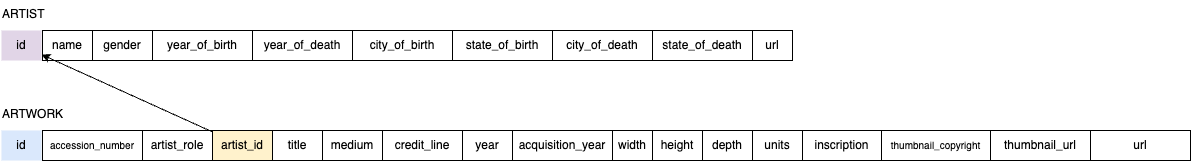
\includegraphics[scale=0.4]{relational_schema.png}
\end{document}